\chapter{Symmetric Key Cryptography}
\label{chap:symmetric}

We now begin our discussion of \gls{symmetriccrypto}.
\Gls{symmetriccrypto} involves one secret key.
This distinguishes it from \gls{publiccrypto}, which we will
discuss in Chapter~\ref{chap:public}, which uses \emph{two} keys:
one public key and one private key.



\section{The Need for Symmetric Key Cryptography}

Alice and Bob would like to communicate with each other
over an \gls{insecure channel}.
In particular, they know that eavesdropper Eve will frequently
be intercepting their communication,
and they do not want her to be find out what they are saying.

Throughout \gls{symmetriccrypto}, we assume that Alice and Bob
have a shared secret key that they can use for communication.
This secret key has been shared through a \gls{secure channel};
in particular, Eve does \emph{not} know what the key is,
although she does know everything about the \gls{encryption scheme}
they are using.
This ensures that Alice and Bob follow
\emph{Kerchoff's principle}~\cite[Page 5]{IntroModernCrypto}:

\begin{quote}
    The cipher method must not be required to be secret,
    and it must be able to fall into the hands of the enemy
    without inconvenience.
\end{quote}

\noindent
The messages that Alice and Bob send to each other shall be called
the \emph{plaintext}.
When the plaintext has been encrypted, the resulting encrypted message
shall be called the \emph{ciphertext} (also spelled \emph{cyphertext}).



\section{Unbreakable Encryption: the One-Time Pad}

\subsection{Definition}

Suppose Alice has a message $m\in\braces{0,1}^{L}$ to send Bob
and wants to encrypt $m$.
Further suppose that Alice previously shared a secret key
$s\chooseRandom{}\braces{0,1}^{L}$ with Bob.
Here, the key $s$ is a uniformly random bit string.
To encrypt $m$ using the \gls{otp}, the ciphertext $c$ is

\begin{equation}
    c \mathDef{} s \oplus m,
\end{equation}

\noindent
where $\oplus$ is the XOR operation.
She then sends the ciphertext $c$ to Bob over an \gls{insecure channel}
(like the Internet).
Because Bob also knows the secret key $s$,
he is able to recover the message $m$ by the XOR operation:

\begin{align}
    s \oplus c &= s \oplus \parens{s \oplus m} \nonumber\\
        &= m.
\end{align}

\subsection{Examples}

We now look at some examples of encryption using the \gls{otp}.

\begin{example}[One-Time Pad 1]
\exampleCodeReference{examples/symmetric/one-time\_pad\_1.py}

We want to encrypt the message

\begin{equation}
    m = \texttt{00112233445566778899aabbccddeeff}
\end{equation}

\noindent
using the \gls{otp} with the secret key

\begin{equation}
    s = \texttt{aa31553ea3fd3f015c4bffac26447514}.
\end{equation}

\noindent
The resulting ciphertext is

\begin{align}
    c &= s \oplus m \nonumber\\
        &= \texttt{aa20770de7a85976d4d25517ea999beb}.
\end{align}

\noindent
Decrypting the message, we see

\begin{align}
    c \oplus s &= \texttt{00112233445566778899aabbccddeeff} \nonumber\\
        &= m,
\end{align}

\noindent
as expected.
See Listing~\ref{list:one-time_pad_1}.

\lstset{
    showstringspaces=false,
    frame=single
}
\lstinputlisting[
    label=list:one-time_pad_1,
    float,
    language=Python,
    caption={Encryption with the \glsentrytext{otp} 1}]{code/symmetric/one-time_pad_1.py}

\end{example}

\begin{example}[One-Time Pad 2]
\exampleCodeReference{examples/symmetric/one-time\_pad\_2.py}

We provide another example of encryption using the \gls{otp}.
Here, we encrypt the same message

\begin{equation}
    m = \texttt{00112233445566778899aabbccddeeff}
\end{equation}

\noindent
using a different secret key:

\begin{equation}
    s = \texttt{09fa37f922072f9cd36cfbc4936d5712}.
\end{equation}

\noindent
A different key produces a different ciphertext:

\begin{align}
    c &= s \oplus m \nonumber\\
        &= \texttt{09eb15ca665249eb5bf5517f5fb0b9ed}.
\end{align}

\noindent
Decrypting the message, we see

\begin{align}
    c \oplus s &= \texttt{00112233445566778899aabbccddeeff} \nonumber\\
        &= m,
\end{align}

\noindent
as expected.
See Listing~\ref{list:one-time_pad_2}.

\lstset{
    showstringspaces=false,
    frame=single
}
\lstinputlisting[
    label=list:one-time_pad_2,
    float,
    language=Python,
    caption={Encryption with the \glsentrytext{otp} 2}]{code/symmetric/one-time_pad_2.py}

\end{example}

\subsection{Discussion}

The \gls{otp} is a \gls{symmetric key encryption} scheme that
\emph{cannot} be broken.
This is called \emph{\gls{perfect security}},
\emph{information-theoretic security},
or \emph{unconditional security}.
Even with \emph{unlimited computation}, the scheme \emph{cannot be broken}.
A proof that the \gls{otp} is perfectly secure can be found
in~\cite[Theorem 2.10]{IntroModernCrypto}.
It is also possible to prove that \gls{perfect security} is possible
only when the total number of keys is greater than or equal
to the total number of messages;
see~\cite[Theorem 2.11]{IntroModernCrypto}.
From this, it follows that any \gls{encryption scheme}
with \gls{perfect security}
must be equivalent to the \gls{otp}

The referenced proofs rely on the fact that $s$ is a uniformly
random bit string the same size of the message.
The secret key $s$ must be \emph{truly random};
anything less is \emph{not sufficient}.
Acquiring true randomness is difficult.
This shows the cost of \gls{perfect security}:
the secret key must be a truly random secret shared beforehand
and the same size as the message.
This is why other \glspl{encryption scheme} are used in practice:
\emph{computational security} enables smaller secret keys.

Anyone who claims to have an unbreakable \gls{encryption scheme} must
either have the equivalent of a \gls{otp} or he is lying;
there are no other possibilities.



\section{Encryption Schemes}

We recall that the primary goal of all \glspl{encryption scheme}
is to convert a plaintext message into a ciphertext which
is indistinguishable from a random bit string.
This random-looking ciphertext is then transmitted over
an \gls{insecure channel}.
Upon receiving the ciphertext, it may be decrypted back into
the original message.

There are two primary classes of \gls{symmetric key encryption} algorithms:
\glspl{stream cipher} and \glspl{block cipher}.
\Glspl{stream cipher} act on the message one bit at a time (in a stream)
while \glspl{block cipher} operate on chunks (or blocks) of bits at a time.

We mention that \glspl{encryption scheme} do not provide
\emph{message integrity};
that is, encrypting a message does not ensure that the message was
not corrupted during transit.
See Chapter~\ref{sec:symmetric_mac} for more information
about message integrity using a \gls{mac}.

The discussion here is meant to give a high-level overview
of \glspl{stream cipher} and \glspl{block cipher}.
The focus is on general ideas,
not current best practices and a thorough description of specific algorithms.
In particular, \emph{do not attempt to write \glspl{encryption scheme}
based on the material presented here.}


\subsection{Stream Ciphers}

Throughout this section, let $L>0$ denote the length of the message in bits.
In general, we will assume that $L$ is significantly larger
than our $k$-bit keys.

\subsubsection{Discussion}

In a certain sense, \glspl{stream cipher} are a natural extension of the
\gls{otp}.
Here, a secret key is stretched into a cryptographically secure
stream of bits.
More formally, let $G:\braces{0,1}^{k}\to\braces{0,1}^{L}$.
Then given a secret key $s\chooseRandom{}\braces{0,1}^{k}$,
the ciphertext is

\begin{equation}
    c = G(s)\oplus m.
\end{equation}

\noindent
Because we are assuming Bob also knows $s$, he can decrypt
the ciphertext:

\begin{equation}
    m = G(s)\oplus c.
\end{equation}

In practice, an \emph{\gls{initialization vector}} may used
in a \gls{stream cipher}.
In this case, we would have
$G:\braces{0,1}^{k}\times\braces{0,1}^{\ell}\to\braces{0,1}^{L}$.
We would then choose the secret key $s\chooseRandom{}\braces{0,1}^{k}$
and \gls{initialization vector} $\textsf{IV}\chooseRandom{}\braces{0,1}^{\ell}$.
The resulting ciphertext would be

\begin{equation}
    c = G(s,\textsf{IV})\oplus m.
\end{equation}

\noindent
In this case, while $s$ must be kept secret,
the \gls{initialization vector} $\textsf{IV}$ is sent
in the clear (unencrypted) along with the ciphertext $c$.
This enables the reuse of the secret key and also ensures
that encrypting the same message under the same secret key
but different \gls{initialization vector} results in a completely different
ciphertext.
Different protocols have different requirements of
\glspl{initialization vector}.
In every case, an \gls{initialization vector} should \emph{never}
be reused.

The important part of a \gls{stream cipher} is the function $G$.
This function must produce an output which is impractical
to distinguish from true randomness.
This should hold for every secret key and \gls{initialization vector}
combination.

\Glspl{initialization vector} are related to \glspl{nonce}.
A \gls{nonce} is a \emph{\textbf{n}umber used only \textbf{once}}.
\Glspl{nonce} should \emph{never} be reused;
\gls{nonce} reuse may \emph{break} the cryptosystem by leaking the private key.

\subsubsection{Examples}

\Glspl{stream cipher} operate on the plaintext in a continuous manner.
Some standard examples include RC4~\cite{rivest2016spritz},
Salsa20~\cite{salsa20}, and ChaCha~\cite{chacha}.
In the case of Salsa20 and ChaCha, the secret key is 256 bits
and the \gls{nonce} is 96 or 64 bits.
RC4 \emph{should not be used} because it is a cryptographically-broken
\gls{stream cipher}~\cite{rfc7465,rivest2016spritz}.


\subsection{Block Ciphers}

\subsubsection{Discussion}

As mentioned previously, a \gls{block cipher} acts on blocks of bits
at a time.
The main property of \glspl{block cipher} is that they are
\emph{keyed} \glspl{permutation}.
We suppose that the secret key is $k$ bits and the block is $n$ bits.
In this case, the \gls{block cipher} would be a function
$E:\braces{0,1}^{k}\times\braces{0,1}^{n}\to\braces{0,1}^{n}$
such that for all $s\in\braces{0,1}^{k}$,
$E\parens{s,\cdot}:\braces{0,1}^{n}\to\braces{0,1}^{n}$
is a \gls{permutation} which appears random.

In order to encrypt a message $m\in\braces{0,1}^{n}$,
Alice chooses a secret key $s\chooseRandom{}\braces{0,1}^{k}$;
Bob receives $s$ through a \gls{secure channel}.
The resulting ciphertext is

\begin{equation}
    c \mathDef{} E(s,m).
\end{equation}

\noindent
Because $E(s,\cdot)$ is a \gls{permutation} (a bijection),
it has an inverse permutation $D(s,\cdot)$.
Thus, Bob can now decrypt the ciphertext to retrieve the plaintext:

\begin{equation}
    m = D(s,c).
\end{equation}

Different methods (called modes) need to be used to encrypt messages
longer than $n$ bits.
There are ways to combine the plaintexts and ciphertexts
to thoroughly scramble the inputs and have the ciphertext
look like a random bit string.
Some modes of operation require the use of an \gls{initialization vector}.

We mention one mode that \emph{should not be used:}
Electronic Codebook (ECB).
It \emph{should not be used} because it does not thoroughly scramble
information.
If we wish to encrypt a message with blocks $m_{1}$, $m_{2}$, and $m_{3}$,
then encrypting with ECB mode would be

\begin{align}
    c_{1} &\mathDef{} E(s,m_{1})
        \nonumber\\
    c_{2} &\mathDef{} E(s,m_{2})
        \nonumber\\
    c_{3} &\mathDef{} E(s,m_{3}),
\end{align}

\noindent
where $s$ is the secret key.
This leaks too much information because, generally speaking,
the message blocks $m_{i}$ will be highly structured.
Also, if $m_{i} = m_{j}$ for $i\ne j$,
then we clearly will have $c_{i} = c_{j}$.
Any secure \gls{block cipher} mode will not leak this information.

\subsubsection{Examples}

Some standard examples of \glspl{block cipher} include
Advanced Encryption Standard (AES)~\cite{FIPS-197-2001},
Data Encryption Standard (DES)~\cite{FIPS-46-3-1977},
Twofish~\cite{TwofishAlg},
and Blowfish~\cite{BlowfishAlg}.
AES has a block size of 128 bits and key sizes of 128, 192, and 256 bits.
DES should not be used because it is a cryptographically-broken
\gls{block cipher}~\cite{rfc4772};
it has a block size of 64 bits and a key size of 56 bits.
AES was in fact designed to replace DES.
Twofish is a \gls{block cipher} designed by Bruce Schneier;
it was a finalist for AES but was not selected as the standard.
Blowfish is old and should not be used;
it was also designed by Schneier.
In 2007, Schneier
\href{https://www.schneier.com/news/archives/2007/12/bruce_almighty_schne.html}{recommended}
switching from Blowfish to Twofish.

As mentioned above, the Electronic Codebook (ECB) mode
\emph{should not be used.}
Instead, consider the algorithm in Figure~\ref{fig:xkcd_cryptography}.

\begin{figure}[t]
\centering
    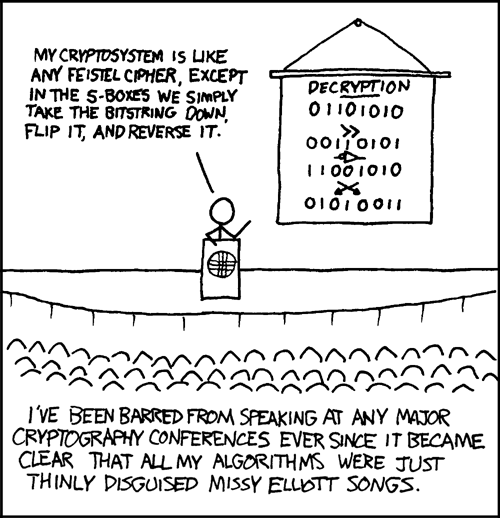
\includegraphics[width=0.75\textwidth]{figures/xkcd/xkcd_153_cryptography.png}
    \caption[\texttt{xkcd} Cryptography]{Here we have an example of
        a \gls{symmetric key encryption} algorithm.
        Created by Randall Munroe on \texttt{xkcd};
        posted online at \url{https://xkcd.com/153/}.
        }
    \label{fig:xkcd_cryptography}
\end{figure}




\section{Cryptographic Hash Functions}

\Glsfirstplural{hash function} are very important in cryptography.
They are discussed in Chapters~\ref{chap:hash}
and \ref{chap:hash_applications}.



\section{Key Derivation Functions}
\label{sec:kdf}

A \emph{\gls{kdf}} (KDF) is a function which takes
a key (perhaps a password, passphrase, or \gls{shared secret})
and uses it to derive \emph{cryptographic} keys.
While the input key material may not be uniformly random bit strings,
the derived cryptographic keys \emph{are} uniformly random bit strings.
This is important because cryptographic protocols usually assume
that the cryptographic keys are uniformly random.
In this way, using the raw input key as a cryptographic key
would decrease the security of the system.

The algorithm \emph{assumes} the input key has sufficient entropy;
problems arise when this assumption is violated.
In practice, a \gls{salt} may also be used so that repeated
input keys produce independent derived keys.
\Glspl{kdf} based on \glspl{hash function} are discussed
in Chapter~\ref{sec:hash_hkdf}.
\Glspl{kdf} may also be used to store passwords.
This aspect is discussed in
Chapter~\ref{sec:hash_apps_password_hashing}.



\section{Cryptographically-Secure Pseudorandom Number Generators}
\label{sec:csprng}

\subsection{Discussion}

In the cryptographic setting, the pseudorandom number generators
that are important are
\emph{\glsfirst{csprng}}
(CSPRNGs).
These are random number generators where it is impractical
to guess the next bit better than average.
This is \emph{not} the case for standard pseudorandom number generators
such as the Linear Congruential Generator~\cite[Chapter 3.2.1]{TAOCP2},
Permuted Congruential Generator~\cite{PCG2014},
or the Mersenne Twister~\cite{matsumoto1998mersenne}.
Their focus is on certain statistical properties and passing
certain statistical tests;
this is necessary but \emph{not sufficient} in cryptography.
In particular, we note that the outputs of LCGs
\emph{fall in planes}~\cite{marsaglia1968random}
and that the internal state recovery of PCGs
is \emph{practical}~\cite{bouillaguet2020practical}.
Also, we note that an
\href{https://cryptopals.com/sets/3/challenges/23}{online challenge}
is devoted to cloning the internal state of the Mersenne Twister
based solely on its outputs.

\Glsfirstplural{csprng} are similar to \glspl{stream cipher}, in that they take
an initial random seed and stretch it into random output.
The difference is that \glsfirstplural{csprng} are able to be reseeded
periodically with additional randomness
so that it is impractical to determine previous outputs.

We mention that even the \emph{notion} of randomness is quite complex
and we will not discuss it further;
one reference for further discussion is~\cite[Chapter 3.5]{TAOCP2}.

\subsection{Examples}

Some examples of \glsfirstplural{csprng} are
Fortuna~\cite[Chapter 10]{PracticalCryptography}\cite[Chapter 9]{CryptoEng},
Hash\_DRBG~\cite[Section~10.1.1]{NIST-SP-800-90ARev1},
and HMAC\_DRBG~\cite[Section~10.1.2]{NIST-SP-800-90ARev1}.
In general, individuals should not worry about specific
\glsfirstplural{csprng} functions.
It should be possible to perform a generic call to retrieve
cryptographically random bits within a cryptographic library;
this is sufficient for normal users.
Do \emph{not} use Dual\_EC\_DRBG~\cite[Section~10.3.1]{NIST-SP-800-90A},
as the standard implementation
is thought to have a backdoor~\cite{BernsteinDualEC}.
See Figure~\ref{fig:xkcd_rng} for another example of a
secure random number generator.

\Glsfirstplural{csprng} are used for constructing private keys,
\glspl{initialization vector}, \glspl{nonce},
and related numbers which need to be drawn from a uniform bit distribution.
They are also used when constructing large prime numbers.

Unless an algorithm has been \emph{specifically designed} to be a
\glsfirstplural{csprng},
it \emph{should not used} when cryptographic random numbers are required.
Otherwise, \href{https://github.com/johguse/profanity/issues/61}{this}
could happen:
\gls{ethereum} private keys could be brute-forced due to insufficient
randomization;
\emph{you have been warned.}

\begin{figure}[t]
\centering
    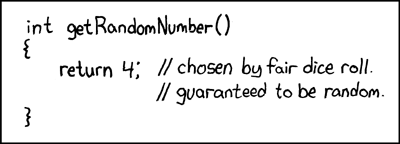
\includegraphics[width=0.75\textwidth]{figures/xkcd/xkcd_221_random_number.png}
    \caption[\texttt{xkcd} RNG]{A secure random number generator
        written in the C programming language.
        Created by Randall Munroe on \texttt{xkcd};
        posted online at \url{https://xkcd.com/221/}.
        }
    \label{fig:xkcd_rng}
\end{figure}




\section{Message Authentication Codes}
\label{sec:symmetric_mac}

\subsection{Discussion}

A \emph{\gls{mac}} (MAC) ensures the integrity
of a message.
This occurs through the use of a shared secret key between parties.

We suppose that Alice and Bob have a shared key used for
message authentication.
In this case, Alice would take her message,
compute a \emph{tag} $t$ using her secret key $k$ and the message $m$,
and send the pair $\parens{m,t}$ to Bob.
Bob would be able to use his copy of the secret key to validate
the pair $\parens{m,t}$.
If the tag is valid, then Bob can be certain that Alice sent him
the message $m$ and that it was not corrupted during transit.

It is important to note that \glspl{mac} do not ensure nonrepudiation;
that is, if Alice sends Bob a message with valid tag,
Bob cannot prove to Charlie that Alice actually sent him the message.
This is because Bob also has access to the (shared) secret key,
and he could have constructed a valid tag for this message.
Additionally, he would have to share his secret key with Charlie
for him to validate the message.
Nonrepudiation is possible with \emph{\glspl{signature}}.
\Glspl{signature} are briefly mentioned in Chapter~\ref{chap:public}
and discussed more thoroughly in Chapter~\ref{chap:signatures}.
We also wish to emphasize that \glspl{mac} do not involve encryption;
in the example above, Alice sent the raw message to Bob.
Combining encryption with message integrity results in
\emph{\gls{ae}} and is discussed
below in Chapter~\ref{sec:symmetric_ae}.

\subsection{Examples}

One example of a \gls{mac} is Poly1305~\cite{poly1305}.
A generic way to build a \gls{mac} is based on a \gls{hash function}:
a \emph{\gls{hmac}}, or HMAC.
HMAC based on the \ShaTwo{} \glsfirst{hash function}
would be written as HMAC-\ShaTwo{}.
The HMAC construction is briefly discussed in Chapter~\ref{sec:hash_hmac};
a more thorough discussion can be found in Appendix~\ref{app:crypto_hmac}.



\section{Authenticated Encryption}
\label{sec:symmetric_ae}

It is important to note that encryption, by itself,
does \emph{not} ensure message integrity;
that is, nothing in the encryption process ensures that
the entire message was correctly delivered.
\emph{\Gls{ae}} is the process of
accomplishing both privacy and integrity
by using an \gls{encryption scheme} with a \gls{mac}.
In practice, this combination is highly desirable.
One example is using the ChaCha20 \gls{stream cipher} and
Poly1305 \gls{mac}~\cite{rfc8439,cryptoeprint:2014:613}.
